尽管DPC++中的向量应该解释为仅适用于单个工作项的工具,但不提到硬件中的SIMD指令是如何操作的话,这一章关于向量的内容就不完整。这个主题并不与向量耦合,而是与向量无关,本书后面描述特定设备类型(GPU, CPU, FPGA)的章节时,就会了解讨论这个话题的重要性了。\par

现代的CPU和GPU包含SIMD指令硬件,对包含在一个向量寄存器或寄存器文件中的多个数据值进行操作。例如,对于Intel x86 AVX-512和其他现代CPU SIMD硬件,SIMD指令可以用来利用数据并行性。在提供SIMD的CPU和GPU上,可以考虑向量加法操作,例如:一个8元素向量上,如图11-13所示。\par

\hspace*{\fill} \par %插入空行
图11-13 SIMD增加了8路数据并行性
\begin{center}
	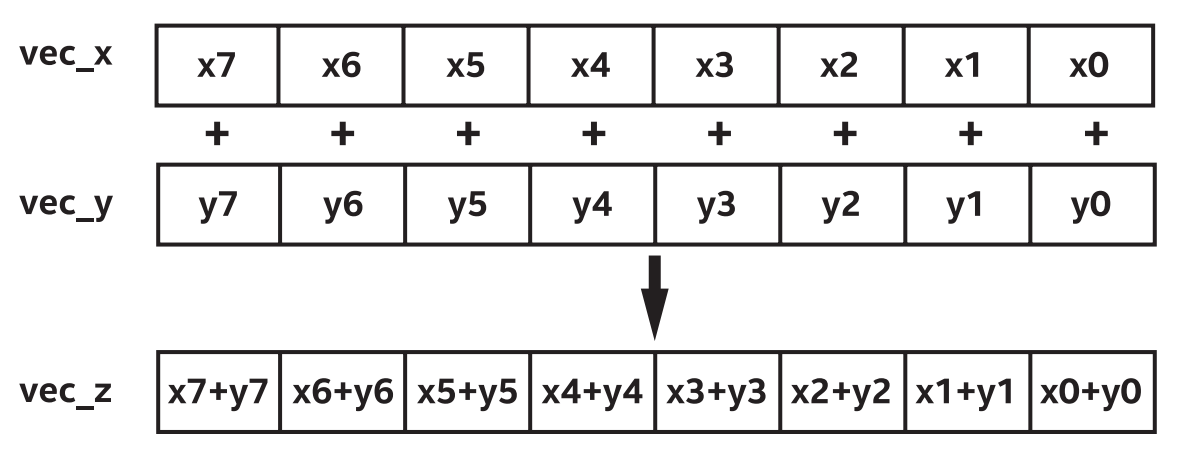
\includegraphics[width=1.0\textwidth]{content/chapter-11/images/2}
\end{center}

本例中的向量加法可以在向量硬件上的一条指令中执行,将向量寄存器vec\_x和vec\_y与SIMD指令并行地相加。\par

以一种与硬件无关的方式公开并行性,确保应用程序可以扩展(或缩小)规模,以适应不同平台的功能,包括那些带有向量指令的平台。在应用程序开发过程中,工作项和其他形式的并行性之间的平衡,是我们必须面对的挑战,这将在第15、16和17章中详细讨论。\par













